\section{Passo 7 — Ligações manuais entre registros}
\label{sec:passo7}

\subsection*{Objetivo}
Corrigir os casos em que a deduplicação automática não reconheceu a mesma invenção em bases
diferentes, ou em que reconheceu duas invenções como uma.

\begin{figure}[H]
\centering
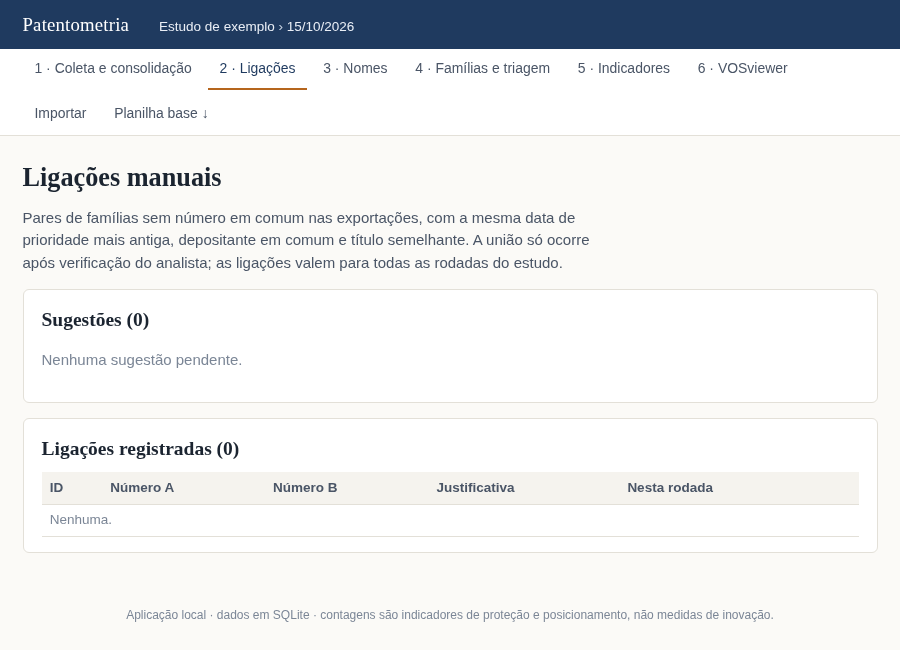
\includegraphics[width=0.9\linewidth]{img/09_ligacoes.png}
\caption{Tela de ligações no estado inicial: nenhuma sugestão e nenhuma ligação registrada. Quando há
pares suspeitos, eles aparecem nesta lista com os números e o motivo.}
\label{fig:ligacoes}
\end{figure}

\subsection*{O que fazer}
\begin{enumerate}
\item Abra \textbf{Ligações}. Leia a lista de sugestões: pares com mesma prioridade, mesmo depositante
      ou título muito próximo.
\item Para cada par, clique em \textbf{Aceitar} (é a mesma família) ou \textbf{Rejeitar} (não é).
\item Se o par não aparecer na lista, registre manualmente os dois números.
\item Volte à rodada e clique em \textbf{Consolidar} novamente para aplicar as ligações.
\end{enumerate}

\subsection*{Como interpretar}
A deduplicação automática usa regras conservadoras: prioridade mais antiga, depositante normalizado e
semelhança de título. Ela erra nos dois sentidos --- deixa de unir famílias quando a prioridade não foi
exportada e une demais quando dois pedidos compartilham prioridade sem serem a mesma invenção.

Aceitar uma ligação \emph{reduz} o número de famílias; rejeitar \emph{aumenta}. Por isso a tela mostra
as ligações aplicadas e as sem correspondência: um número grande de sem correspondência costuma
indicar número digitado errado ou formato de publicação diferente entre bases.

\begin{nota}[Ligação é decisão de estudo]
As ligações valem para o estudo inteiro, não para uma rodada. Ao repetir a coleta, elas continuam
valendo; revise-as quando o corpus mudar de escopo.
\end{nota}

\begin{alerta}[Erro comum]
Editar a ligação e não reconsolidar. Sem a reconsolidação, o PRISMA continua com os números antigos e
a decisão parece não ter efeito.
\end{alerta}

\subsection*{Checkpoint}
\marcador\; O número de famílias muda depois da reconsolidação e as ligações aparecem como ``aplicadas''.
